\documentclass[11pt]{article}

\usepackage[doublespacing]{setspace}
% \usepackage[margin=1in]{geometry}

\usepackage{fancyvrb}
\usepackage{lipsum}
\usepackage{cite}
\usepackage{graphicx}


\title  {``Bees?''\\ A Large Scale, Co-operative Simulation 
         Weighing Altruism and Selfishness}
\author {Alexander Simms, Ravenna Thielstrom}
\date   {CS 81: Adaptive Robotics, Spring 2014}
\begin{document}
	\maketitle

	\begin{abstract}
		% A short abstract of 200 to 300 words summarizing your findings. 

		The Prisoner’s Dilemma, in philosophy, is a hypothetical situation that tests human nature. Two criminals are imprisoned. If, however, one prisoner should choose to defect and betray the other, he will be set free and the betrayed prisoner will receive 3 years of prison. If, on the other hand, they simultaneously betray each other, both will receive a 2 year sentence. Cooperative silence from both parties gets them both a lesser sentence of 1 year. Although a human may argue that altruism is the best option for both parties, game theory states that in this situation, one should always choose to betray in order to minimize personal loss, and indeed one would expect this kind of decision from an artificial agent. Yet plenty of communities exist in nature that revolve around altruistic cooperation- for example, a bee colony, where individual bees retrieve nectar for the communal hive rather than scouting selfishly for their own survival. Although cooperation can certainly be implemented into an artificial life simulation, from an evolutionary standpoint a more interesting question is raised: can the interactions of a group and the parameters of their environment produce emergent cooperation among independent agents? This research aims to investigate the possibility of emergent altruism through evolutionary game theory. To this effect, we used NEAT to evolve neural-net topologies across many generations in a bee colony simulation, testing what possible circumstances might lead to altruistic decisions or selfish decisions in the hive. Initial speculation produced a hypothesis that the amount of altruism and selfishness demonstrated in NEAT-trained agents will be most affected by an individual fitness relying on group fitness. However, the results of our experiments demonstrate that while this is partly true and group fitness is key to altering artificial behavior, in the end selfishness wins out.


	\end{abstract}

	\section{Introduction} % (fold)
	\label{sec:introduction}
		% An introduction that contrasts your study with other related work. 
		% Find and read at least three articles related to your experiment and 
		% discuss these papers here. 
		
		Cooperative behavior has frequently been discussed within the contexts of artificial intelligence. The Prisoner's Dilemna itself often serves as a basis for these discussions due to its relevance to issues of social order and the challenges thereof. Michael W. Macy's paper on ``Social Order in Artificial Worlds'' describes the Prisoner's Dilemna as the ``paradox of social order''. \cite{macy} Macy specifically names four possible outcomes in the Prisoner's Dilemna, ordered by the amount of payoff: temptation (defecting while the other prisoner remains silent), reward (both prisoners staying silent), punishment (both prisoners defect), and sucker (staying silent while the other prisoner betrays you). The reason why this game can be called a paradox is that the choice leading to the highest payoff (selfishness) also has the potential for the greatest failure. Since our experiments take place not on an individual-to-individual level but rather in a large hive-type colony, our experiments don't explicitly use the Prisoner's Dilemna. However, each agent has a similar choice of selfishness or altruism with similar ordered outcomes, only on a larger communal scale:
		\begin{itemize}
		\item Temptation: selfish agents receive a random (potentially above average) fitness
		\item Reward: altruistic agents receive an average fitness
		\item Punishment: enough agents are selfish that hive fitness drops for all
		\item Sucker: a minority of agents behave altruistically while a majority behave selfishly, reducing hive fitness for all
		Unlike the true Prisoner's Dilemna, instead of temptation/sucker and reward/punishment being linked, our experiment has temptation/reward and punishment/sucker linked. Also, punishment and sucker potentially receive the same amount of low payoff. This could supposedly lower the potential for selfishness since acting altruistically no longer possibly leads to a worse ending than acting selfishly.

		As mentioned by Macy, the single-iteration Prisoner's Dilemna is best played with a selfish dominant strategy, according to game theory. Our experiments show the same, for reasons discussed later. However, this strategy is not the best when the Prisoner's Dilemna is repeated, as expanded upon in David B. Fogel's ``Evolving Behaviors in the Iterated Prisoner's Dilemna'' \cite{fogel}. A recurrent Prisoner's Dilemna is often effective because players will learn over time which individuals are more likely to defect or cooperate, and adjust their strategies accordingly when facing each of those individuals. However, in a hive environment where many independent agents are making the decision simultaneously, this is not a viable option to learn. Instead, the value of implementing a recurrent network in our experiments comes from the knowledge of the previous iteration, potentially informing the 



	% section introduction (end)

	\section{Experiments} % (fold)
	\label{sec:experiments}
		% A detailed description of your experiments. 
		% There should be enough information provided so that someone could 
		% reproduce your experiments. 

		\subsection{The Bee Model} % (fold)
		\label{sub:the_bee_model}
			To conduct these experiments, a model was developed that takes inspiration from the nectar-collecting hive insect, known in some circles as the bee. Our model consists of a population of individual neural nets, evolving by the NeuroEvolution of Adapting Topologies algorithm, henceforth referred to as NEAT.\cite{neat} NEAT, first developed by the illustrious Kenneth O. Stanley, is a genetic algorithm that has a flexible genetic encoding that allows for the topology of the network to grow and change over time, based on a user-defined measure of ``fitness''. All of the genes within the genetic encoding are tagged with historical markings, which allows for quick implementation of ``crossing-over,'' the process by which genetic information from an individual's parents is mixed. Finally, NEAT allows for speciation: individuals within the population are grouped together based on the similarness of their genomes, and only those individuals with similar genomes are allowed to reproduce. This allows for each species to find its own niche, and prevents any one species from outcompeting all of the others. It is because of these features that NEAT was selected for this task.

			Each individual NEAT agent within this model is called a ``bee'', and the population of all of the NEAT agents is called the ``hive''. Each ``day'' within this model, all of the bees leave the hive to go and find nectar. The nectar is represented in this model as a random floating-point number between 0 and 1. When it recieves this nectar, it has the choice to either be selfish or altruistic. If the bee decides to be selfish, it eats the nectar then and there. If it decides to be altruistic, it brings the nectar back to the hive, where all of the nectar brought back by altruistic bees is pooled and shared equally among all of the altruistic bees. The ``fitness'' in this system is simply how much nectar a bee was able to eat on a given day.
		% subsection the_bee_model (end)

		\subsection{Basic Experiment} % (fold)
		\label{sub:basic_experiment}
			An experiment was carried out to determine the workability of the model. In this experiment, each bee lived for only one day, and afterwards died. Their fitnesses determined the makeup of the next generation of bees: the most fit bees were bred to produce hopefully more fit offspring. The NEAT network evolved with the settings described in Appendix \ref{sub:configuration_for_basic_experiment}. Its only input was the nectar it found, again, a float between 0 and 1, and output represented the choice it made. (See Figure \ref{fig:naive_system}.)

			\begin{figure}[tb]
				\begin{center}
					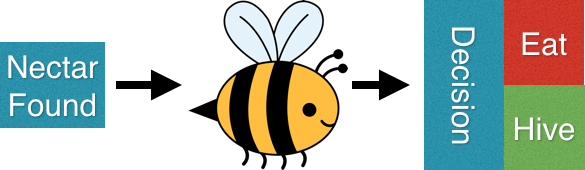
\includegraphics[scale=.5]{bee_diagrams/naive_system.png}
				\end{center}
				\caption{All that is fed into the system is the amount of nectar that the bee has found on that day, and the choice that the bee has made is determined by whether the output is closer to 0 or to 1.}
				\label{fig:naive_system}
			\end{figure}

			\begin{figure}[tb]
				\begin{center}
					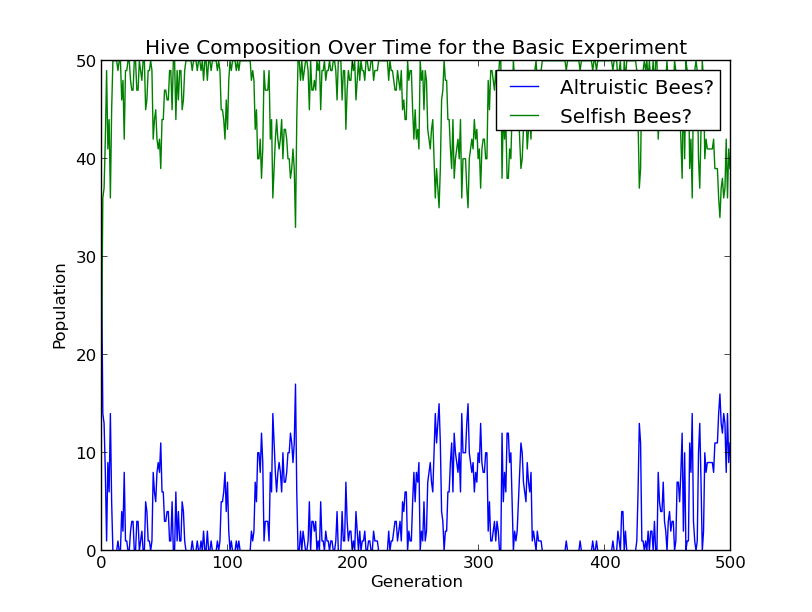
\includegraphics[scale=.5]{results/basic_comp.png}
				\end{center}
				\caption{Under the conditions of the basic experiment, altruism lost handily to selfishness.}
				\label{fig:basic_experiment_composition}
			\end{figure}

			In all of the trials run, the majority of the bees wound up selfish. A representative trial is shown in Figure \ref{fig:basic_experiment_composition}. There are a number of reasons for this, the most pressing being the fact that the bees had no direct incentive to act altruistically. While more stable fitnesses could theoretically be obtained through altruism, the system only works if a all of the bees are acting altruistically: enough bees will bring back above-average amoutns of nectar to offset the bees that bring back a below-average aomunt of nectar. However, if too few bees are acting altsuistically, then this buffering effect is not present. 


		% subsection basic_experiment (end)

		\subsection{Hive Fitness} % (fold)
		\label{sub:hive_fitness}
			How, then, can this selfishness be subverted? Well, in the real world, actual hives collect the nectar that the bees bring in, and convert it in to honey. This is the inspiration for a measure of ``hive fitness,'' which we have implemented as an integer between 0 and 10, indicating how much nectar the hive has on ``reserve''. Each day, when the altruistic bees bring the honey back, a tenth of the honey is taken from them and put into the hive, to support the ``queen,'' who eats 0.5 units of nectar per day. The amount of nectar in the reserve is turned into a modifier as described in Figure \ref{fig:modifier_algorithm}, which is then multiplied by the amount of nectar each bee finds to determine their fitness.

			\begin{figure}[tb]
				%% HERE THERE BE DRAGONS:
				%% The verbatim environment is indented with spaces because
				%% the Verbatim environment is stupid.
				\begin{Verbatim}[frame=single]
                if hive_nectar > 10:
                    modifier = 1
                elif hive_nectar > 0:
                    modifier = hive_nectar / 10
                else:
                    modifier = .00001 
				\end{Verbatim}
				\caption{The fitness of each bee is affected by the amount of nectar reserves in the hive. The modifier defined by this section of code is multiplied by the amount of nectar the bee collected in order to determine that bee's fitness.}
				\label{fig:modifier_algorithm}
			\end{figure}

			\begin{figure}[tb]
				\begin{center}
					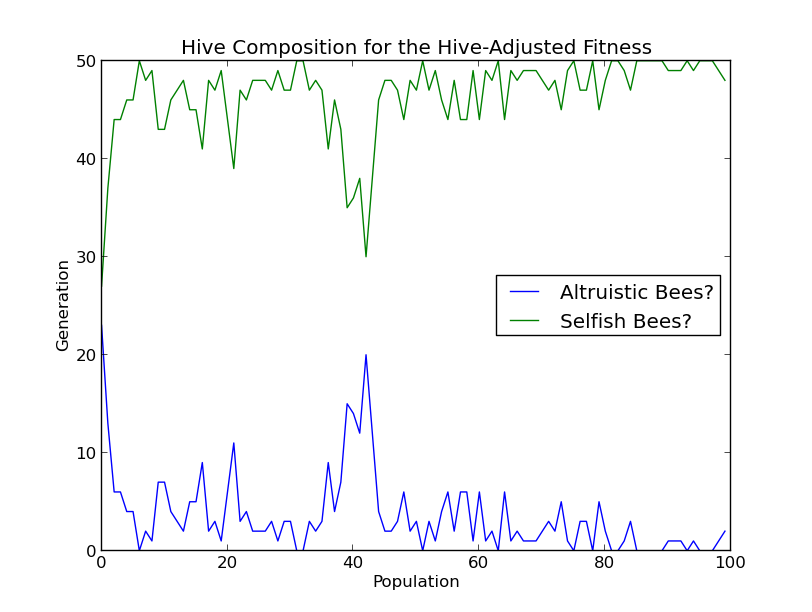
\includegraphics[scale=.5]{results/hive_fitness_comp.png}
				\end{center}
				\caption{OH GOD}
				\label{fig:figure1}
			\end{figure}

			\begin{figure}[tb]
				\begin{center}
					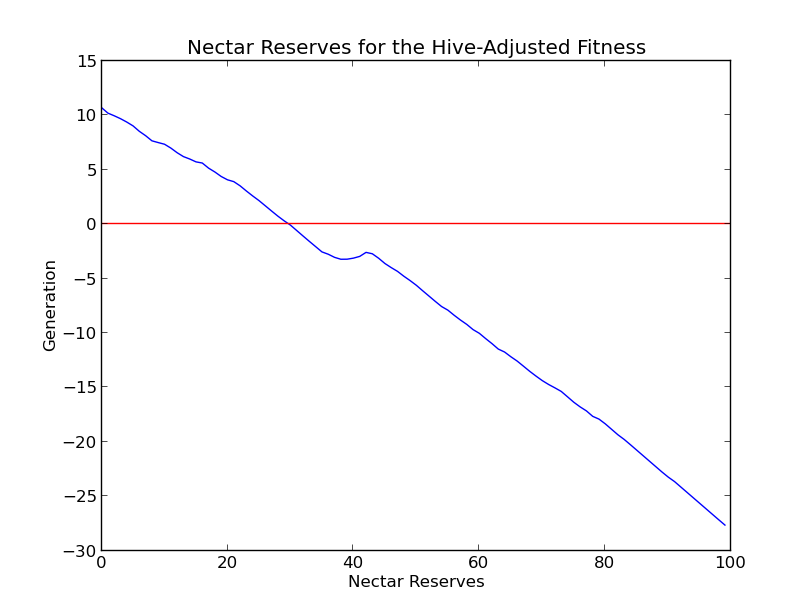
\includegraphics[scale=.5]{results/hive_fitness_res.png}
				\end{center}
				\caption{Caption here}
				\label{fig:figure1}
			\end{figure}
		% subsection hive_fitness (end)

		\subsection{Recurrent Networks} % (fold)
		\label{sub:recurrent_networks}
		\lipsum[12-14]
		% subsection recurrent_networks (end)

		\subsection{Advice from Bees} % (fold)
		\label{sub:advice_from_bees}
		
		% subsection advice_from_bees (end)

	% section experiments (end)

	\section{Discussion} % (fold)
	\label{sec:discussion}
		One substantial difficulty for the development of altruism comes from the way that the fitness function is implemented. Rll of the bees coming back are coming back with nectar in the range of 0 and 1, so amortized, choosing to be altruistic is choosing a fitness of $0.5$.Choosing to be selfish has the potential to obtain much higher
		fitnesses than that, and those individuals will be able to reproduce.
	% section discussion (end)
	\singlespacing
	\appendix
	\pagebreak
	\section{NEAT Configurations} % (fold)
	\label{sec:neat_configurations}
	
		\subsection{Configuration for Basic Experiment} % (fold)
		\label{sub:configuration_for_basic_experiment}
			\begin{verbatim}
				[phenotype]
				input_nodes         = 1
				output_nodes        = 1
				max_weight          = 30
				min_weight          = -30
				feedforward         = 0
				nn_activation       = tanh 
				hidden_nodes        = 0
				weight_stdev        = 0.9

				[genetic]
				pop_size              = 50
				max_fitness_threshold = 1

				# Human reasoning
				prob_addconn          = 0.05
				prob_addnode          = 0.03
				prob_mutatebias       = 0.2
				bias_mutation_power   = 0.5
				prob_mutate_weight    = 0.9
				weight_mutation_power = 1.5
				prob_togglelink       = 0.01
				elitism               = 1

				[genotype compatibility]
				compatibility_threshold = 3.0
				compatibility_change    = 0.0
				excess_coeficient       = 1.0
				disjoint_coeficient     = 1.0
				weight_coeficient       = 0.4

				[species]
				species_size        = 10
				survival_threshold  = 0.2
				old_threshold       = 30
				youth_threshold     = 10
				old_penalty         = 0.2
				youth_boost         = 1.2
				max_stagnation      = 15
			\end{verbatim}
		% subsection configuration_for_basic_experiment (end)

		\pagebreak
		\subsection{Configuration for Hive Fitness} % (fold)
		\label{sub:configuration_for_hive_fitness}
			\begin{verbatim}
				[phenotype]
				input_nodes         = 1
				output_nodes        = 1
				max_weight          = 30
				min_weight          = -30
				feedforward         = 0
				nn_activation       = tanh 
				hidden_nodes        = 0
				weight_stdev        = 0.9

				[genetic]
				pop_size              = 50
				max_fitness_threshold = 1

				# Human reasoning
				prob_addconn          = 0.05
				prob_addnode          = 0.03
				prob_mutatebias       = 0.2
				bias_mutation_power   = 0.5
				prob_mutate_weight    = 0.9
				weight_mutation_power = 1.5
				prob_togglelink       = 0.01
				elitism               = 1

				[genotype compatibility]
				compatibility_threshold = 3.0
				compatibility_change    = 0.0
				excess_coeficient       = 1.0
				disjoint_coeficient     = 1.0
				weight_coeficient       = 0.4

				[species]
				species_size        = 10
				survival_threshold  = 0.2
				old_threshold       = 30
				youth_threshold     = 10
				old_penalty         = 0.2
				youth_boost         = 1.2
				max_stagnation      = 15
			\end{verbatim}
		% subsection configuration_for_hive_fitness (end)

		\pagebreak
		\subsection{Configuration for Recurrent Networks} % (fold)
		\label{sub:configuration_for_recurrent_networks}
			\begin{verbatim}
				[phenotype]
				input_nodes         = 4
				output_nodes        = 1
				max_weight          = 30
				min_weight          = -30
				feedforward         = 0
				nn_activation       = tanh 
				hidden_nodes        = 0
				weight_stdev        = 0.9

				[genetic]
				pop_size              = 50
				max_fitness_threshold = 1

				# Human reasoning
				prob_addconn          = 0.05
				prob_addnode          = 0.03
				prob_mutatebias       = 0.2
				bias_mutation_power   = 0.5
				prob_mutate_weight    = 0.9
				weight_mutation_power = 1.5
				prob_togglelink       = 0.01
				elitism               = 1

				[genotype compatibility]
				compatibility_threshold = 3.0
				compatibility_change    = 0.0
				excess_coeficient       = 1.0
				disjoint_coeficient     = 1.0
				weight_coeficient       = 0.4

				[species]
				species_size        = 10
				survival_threshold  = 0.2
				old_threshold       = 30
				youth_threshold     = 10
				old_penalty         = 0.2
				youth_boost         = 1.2
				max_stagnation      = 15
			\end{verbatim}
		% subsection configuration_for_recurrent_networks (end)
	% section neat_configurations (end)

	\nocite{*}
	\bibliography{bib}
	\bibliographystyle{plain}

\end{document}